\subsection{Session 2, Exercise 10}

\lineparagraph{Exercise}

Let $\Sigma = \{0, 1\}$. The sequences are considered as binary numbers. Give a finite automaton that accepts exactly those words that represent numbers divisible by three in binary form. Take into consideration that a number does not begin with $0$, except for number zero itself, and that the input number is read beginning with the most significant digit.

\lineparagraph{Solution}

Any automaton that we design will work by reading the input binary string from left to right. We will want to keep track of the remainder of the current binary number after each 0 or 1 we read. The question is how do we update this remainder when the next input character comes? First, let's do a simpler task, just keeping track of the number itself and updating it as we go.

\begin{itemize}
    \item For example, let's say that so far we have read the the ''$101$'' binary string on the input. That is a $5$ in decimal form.
    \item Let's say the next character is also a $1$, so now the current string is ''$1011$'', or in decimal form $11$.
    \item This was achieved by shifting the string ''$101$'' to the left and adding a ''$1$'' as the least significant character.
    \item A left shift in binary corresponds to multiplication by $2$ in decimal, and then if the next character is a $1$, we just need to add $1$ to the decimal value as well. So in our example, $5*2 + 1 = 11$.
    \item In general, if we read a binary number from left to right, to calculate its decimal value, we simply multiply the current decimal value by $2$, and if the bit we read was a $1$, we add a $1$ and continue to the next bit.
\end{itemize}
 
If we don't care about the entire number, just its remainder when divided by $3$, we can do the same calculation, but modulo $3$.

If the current number is divisible by $3$, or in the form $3k$, and the next binary character is a $0$, then to update we do $3k*2+0 = 6k$, which means that the updated number will still be divisible by $3$.

If the next binary character is a $1$, then to update we do $3k*2+1=6k+1=3*(2k)+1$, which means that the updated number has a remainder of $1$ when divided by $3$.

We can represent these statements by the following two transitions from state $3k$:

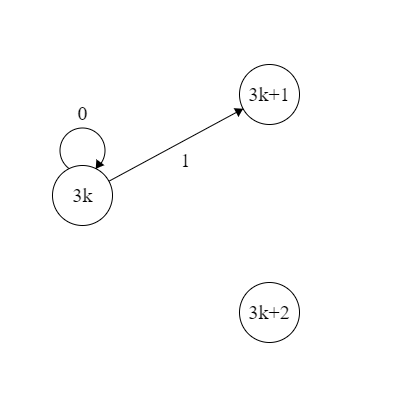
\includegraphics[width=250px]{02/modulo_1.png}

If the current number has a remainder of $1$, when divided by $3$, or in the form of $3k+1$, and the next binary character is a $0$, then to update we do $(3k+1)*2+0=6k+2=3*(2k)+2$, which means that the updated number has a remainder of $2$, when divided by $3$.

If the next binary character is a $1$, then to update we do $(3k+1)*2+1=6k+3=3*(2k+1)$, which means that the updated number is divisible by $3$.

We can represent these statements by the additional two transitions from state $3k+1$:

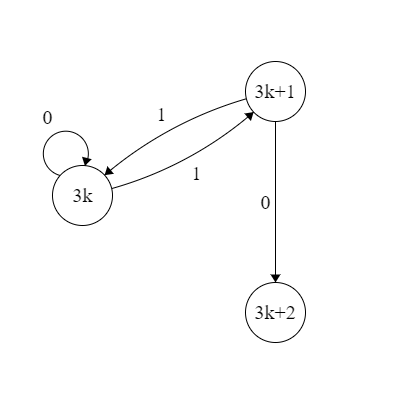
\includegraphics[width=250px]{02/modulo_2.png}

Finally, if the current number has a remainder of $2$, when divided by $3$, or in the for of $3k+2$, and the next binary character is a $0$, then to update we do $(3k+2)*2+0=6k+4=3*(2k+1)+1$, which means that the updated number has a remainder of $1$, when divided by $3$.

If the next binary character is a $1$, then to update we do $(3k+2)*2+1=6k+5=3*(2k+1)+2$, which means that the updated number has a remainder of $2$, when divided by $3$.

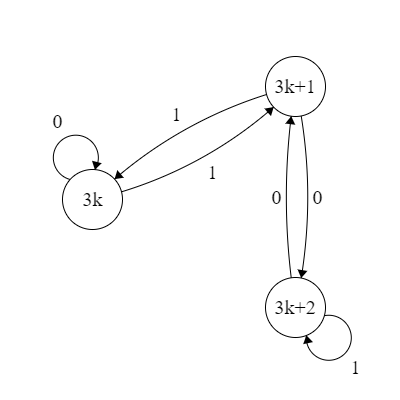
\includegraphics[width=250px]{02/modulo_3.png}

If you want to try this automaton, come up with any decimal number, turn it into binary form and calculate its remainder by $3$, by applying the transitions above using its binary form as input. The starting state should be $3k$, since when we have not read anything in yet, so we want to start from a state that is equivalent to the number $0$, which is divisible by $3$.

I however, did not mark a starting state yet on this image, because there is one additional statement to keep in mind: ''Take into consideration that
a number does not begin with $0$, except for number zero itself.''. This means that we do not consider any string longer than 1 characters starting with a $0$ a number, much less a number that is divisible by $3$, so we need to reject these words.

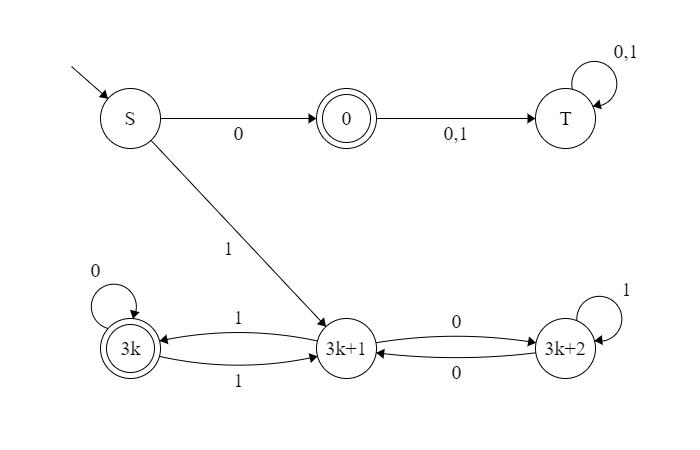
\includegraphics[width=\linewidth]{02/modulo_final.png}

Now, if this was an exam, here is how to prove that this accepts the language: (Basically everything I just said, but in a shortened form.)

\textbf{Proof:}

1. Let's explain what the different states mean and that their transitions are correct:

\begin{itemize}
    \item $S$ is the starting state. If we read a $0$ in, we move to a state dedicated to the number $0$. If we read a $1$ in, we move to the state that represents binary numbers, that give a remainder of $1$ when divided by $3$, which is true for the (binary) number $1$.
    \item The only word for state $0$ is $0$ itself, this is divisible by $3$ and is accepted. If we read anything else after a $0$ that is an incorrectly formatted number and moves to a trap state $T$ which rejects it.
    \item The states $3k$, $3k+1$ and $3k+2$ represent the 3 remainder classes of division by $3$. When a new character is read on the input, we update the remainder class with multiplying by $2$ (binary shift) and adding the $0$ or $1$ bit we just read. We can see that the transitions are correct, since:
    \begin{itemize}
        \item $3k*2+0 = 3*(2k)$
        \item $3k*2+1 = 3*(2k)+1$
        \item $(3k+1)*2+0 = 3*(2k)+2$
        \item $(3k+1)*2+1 = 3*(2k+1)$
        \item $(3k+2)*2+0 = 3*(2k+1)+1$
        \item $(3k+2)*2+1 = 3*(2k+1)+2$
    \end{itemize}
\end{itemize}

2. Let's explain that the correct words are accepted and the words not in the language are rejected:

The words in the language are any numbers that are divisible by $3$, which is either the number $0$ or anything that is in the form $3k$, these states are accepting.

A word could be outside of the language due to being malformed (starting with $0$, but not being $0$ itself), which will be redirected to a trap $T$; or due to not being divisible by $3$, in which case it will land in either $3k+1$ or $3k+2$ and will be rejected there. Finally, the empty string is rejected because it's not a number, which is the only word that will end up in state $S$.

\textbf{(End of proof.)}

Notes:

\begin{itemize}
    \item I ended up making a deterministic automaton here, however the task would allow a non-deterministic one as well. We could get rid of the enitre $T$ state and define no transitions outwards from state $0$. If there is input left to be read in state $0$ the automaton halts due to a missing transition, which rejects the word regardless of the accept/reject status of the current state!
\end{itemize}